% chap1.tex {Introductory Chapter}

\chapter{Introduction}
This work is an early step towards fascilitating interdisciplinary research within the University of Texas at El Paso.
In the future, we wish to design a system to automatically assign or recommend faculty to
interdisciplinary research communities based on their publication data. For this task, we want to learn models that capture
important and high-level features from raw text in order to make decisions as accurate and meaningful to the faculty members as possible.
Neural networks are effective at learning said complex features. One important consideration is that neural networks work best when trained
using large amounts of data, as is the case with statistical models.
This study is to better understand deep convolutional and recurrent networks for the task of classifying scientific publication abstracts and how
well they can cope with limited amounts of data. We evaluate the predictive performance of multiple types of neural networks for text classification.
We then evaluate the effect of integrating distributed representations of words as free parameters of the model. We then propose several data augmentation techniques to help reduce the effects caused by our
moderate-sized training set.

\section{Text Classification}
Text classification is the task of assigning a label to a text document. A document can be any piece of text we wish to process; in this
work, we label scientific and engineering publication abstracts. We wish to create a \textbf{model} that parametrizes
some function that labels a document based on its \textbf{features}. The features of a document can be any set of values
computed from the document itself. These features are the input representation used for our classification model. A very popular feature representation of documents is the
\textit{\textbf{term frequency}}-\textit{\textbf{inverse document frequency}} (tf-idf) representation, where a document is represented as a vector of frequency-based statistics of its words \cite{luhn1957statistical}.
Another popular feature representation of documents is the \textit{\textbf{Bag-of-Words}}(BoW) representation, where a document is represented as a vector of indexes,
each index corresponding to a word in the document \cite{joachims2002learning}. A more recent approach to text classification is to use neural networks to automatically
extract high-level features that contain context and semantic information \cite{johnson2014effective}\cite{graves2013speech}. In the following sections, we
describe neural networks and provide a general overview of how to train them to allow generalization for tasks such as text classification.



\section{Neural Networks}
A neural network is a function $f(\bm{x};\bm{\theta})$ that maps an input $\bm{x}$ to some response variable $y$.
Neural networks are commonly represented as directed acyclical graphs. Each node is called a hidden unit, namely because it computes a latent variable of its input.
We compute a unit's output as the dot-product of inputs with a corresponding set of parameters, followed by a non-linear function applied to the resulting scalar.
This non-linearity is referred to in machine learning as the unit's \textit{activation} function. This process is called \textbf{forward propagation}, or a forward pass of the
neural network. Given input vector $\bm{x}$, we forward-propagate to compute the the $i$th hidden unit's output as:
\[h_i = g(\bm{x} \cdot \bm{\theta} )\]
where $g$ is a non-linear activation function.
\begin{figure}[H]
\centering
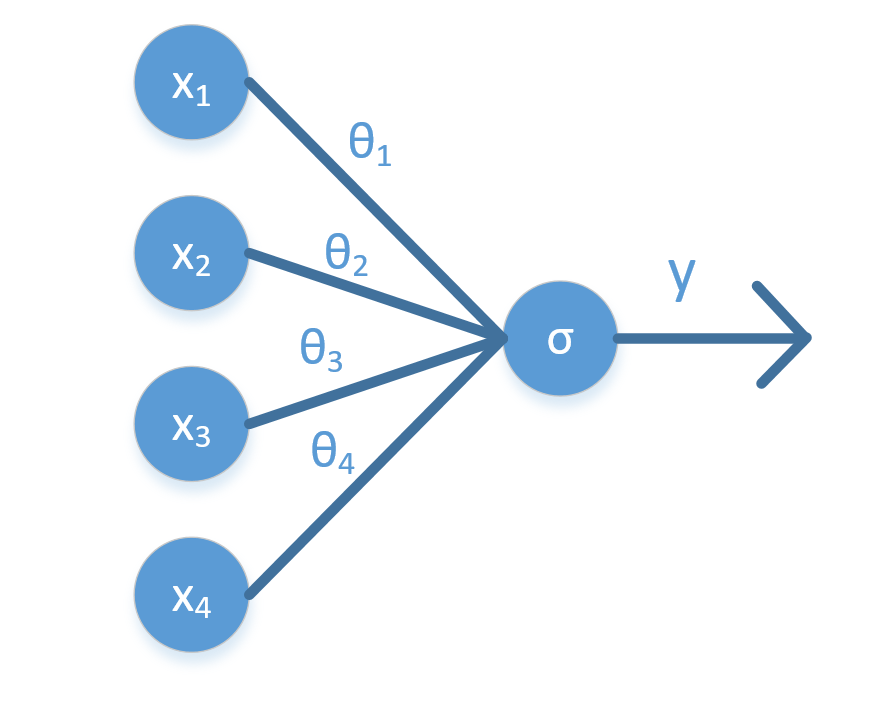
\includegraphics[width=0.5\textwidth]{MLP.png}
\caption{Visualization of a single unit neural network. A non-linearity is applied to the linear combination of the
inputs $x_i$ with the weights $\theta_i$.}
\end{figure}
When we \textit{train} a
neural network, we \textit{learn} the model parameters, or weights, $\bm{\theta}$ that minimize some cost function $J(\bm{\theta})$.
For a regression task, where the model's output is a continuous variable, a common cost function is the \textbf{Mean Square Error}:
\[J(\bm{\theta}) = \frac{1}{m}\sum_{i=1}^{m}(y_{i} - f(\bm{x}_{i};\bm{\theta}))^{2}\]

For categorical or discrete output variables found in classification tasks, we normally use the \textbf{Categorical Cross-Entropy}:

\[J(\bm{\theta}) = -\mathbb{E}_{\bm{x},y \sim \hat p_{data}} \log \textit{p}(y|\bm{x};\bm{\theta})\]

Given a \textit{training} set of observations $\bm{x}_i$ and their true labels $y_i$, we compute weights that minimize the cost, or error, via
maximum likelihood (ML) estimation:

\[\bm{\theta}_{ML} = \argmax_{\bm{\theta}} \sum_{i}^{m} \log P(y_{i}|\bm{x}_{i};\bm{\theta})\],

which one can see is equivalent to computing the weights that \textbf{\textit{minimize}} the cross-entropy cost function.


\subsection{Minimizing Non-Convex Functions: Gradient-Based Learning}
Due to the non-linearities associated with a neural network, the loss function to be minimized becomes non-convex.
Non-convex optimization is in general more difficult than convex optimization, so we usually rely on gradient-based methods for the task.
Gradient based optimization provides a sound theoretical framework and a practical and well tested methodology for learning
deep neural networks. This gradient-based learning process involves \textit{moving},
or updating, the weight values in the direction opposite of the cost function's gradient, repeating this process for a series of
\textbf{epochs}, or training iterations.
These updates should be small, scaled by a
\textit{learning rate}, and can make learning a lengthy process. Gradient based learning is also scalable to datasets of enourmous size.
The gradients and updates may be computed using small random batches of the training set at a time rather than the entire dataset; this is known as Stochastic Gradient Descent \cite{bottou2010large}.

\subsection{Bias-Variance Tradeoff}

Given a set of identically and independently distributed observations $\{\bm{x}_1, ... , \bm{x}_n\}$, we wish to compute the set of
weights $\bm{\hat{\theta}}$ that is as close as possible to $\bm{\theta}$, the set of weights that truly parametrize the data generating
process $p_{data}(\bm{x};\bm{\theta})$ and thus minimizes the cost function. This concrete set of parameters (in contrast to a density over
possible values) is called a \textbf{point estimator}, or statistic, of the true set of parameters.
Unless the data generating process is known exactly, the parameter estimators will have error.
Two different measures of error in an estimator are its bias and variance.
The \textbf{bias} measures the expected deviation between $\bm{\theta}$ and the estimator $\bm{\hat{\theta}}$,
with this expectation being over the data:

\[Bias(\bm{\hat{\theta}}) = \mathbb{E}{(\bm{\hat{\theta}})} - \bm{\theta}\]
\[ = \mathbb{E}{[\bm{\hat{\theta}} - \bm{\theta}}]\]
Intuitively the bias can be viewed as error caused by generalization in the model. If a model is trained with high bias, it will make strong assumptions
of the data generating process. For example, it can assume that the \textbf{decision boundary}, or region of separation between classes, is linear when it could be quadratic.

The \textbf{variance} is a measure of the deviation from the expected estimator, caused by
the randomness in the sample, or how much the estimator will vary as a function of the data sample:

\[ Var(\bm{\hat{\theta}}) = \mathbb{E}{[\bm{\theta} - \bm{\hat{\theta}}]^{2}}\]

Intuitively, the variance can be seen as error caused by variation in the training set; how much will the set of parameters differ from its expected value given a different training sample.
Thus, if a model is trained with high variance, it will learn to model the nuances and variations specific to the training sample with low error but will fail to generalize well to new, unseen test data.
During training, we obtain $\bm{\theta}_{ML}$ by minimizing $J_{train}(\bm{\theta})$, but we care about having low $J_{test}(\bm{\theta})$, or low cost
on test data points. We seek a model that has a balance between variance (training specific nuances) and bias (generalization). This is known as the bias-variance tradeoff.

\begin{figure}[H]
\centering
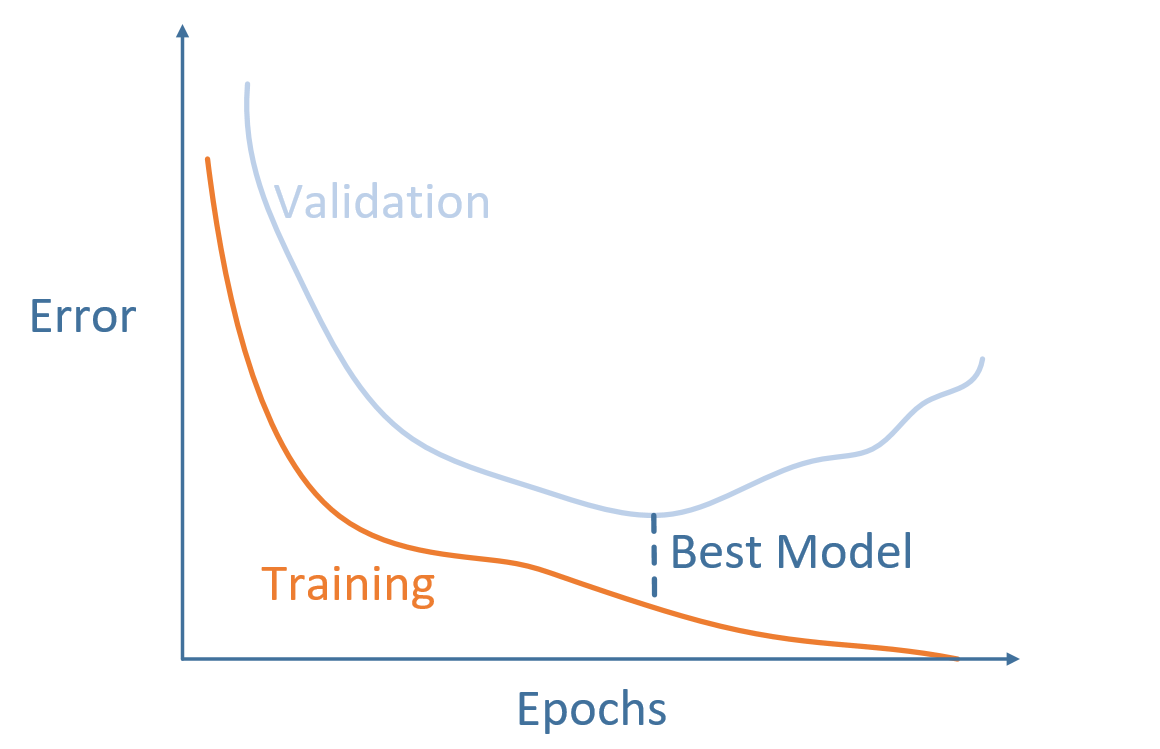
\includegraphics[width=0.5\textwidth]{OverfittingLossPlot.png}
\caption{Visualization of overfitting. Training error decreases as epochs progress, eventually reaching zero.
Validation error starts increasing, indicating overfitting. The best model is shown at the dotted line, where
validation error reached its minimum.}
\end{figure}

\textbf{Overfitting} occurs when a network is able to predict its training set extremely well (i.e. very close to zero error), but fails to predict
unseen data points. This is because the network's weights have been extremely fine-tuned to \textit{fit} its training data, but do not fit or represent
data points outside of its training samples.
An overfitted model is said to have large \textbf{variance} and small \textbf{bias}. Conversely, underfitting occurs when the model fails to predict
the training set because it generalizes too much. This model is said to have large bias and small variance. When training a neural network,
we aim to find a balance between training cost and test cost, between overfitting and underfitting.

Because of the commonly large number of weights in deep convolutional networks, it is easy to overfit a moderate size training set \cite{hinton2012improving}.
It has been shown that when using a large enough dataset, neural networks are trained without overfitting, and thus generalize well
to new unseen data. Because of the abundance of data today, it is usually easy to acquire large datasets, although this is not always the case.
In this work, we consider the case when the available datasets are of moderately size, for example tens of thousands of examples.

\subsection{Weight Regularization}
One way to regularize a model is to impose a constraint on its weights. By adding a penalty term based to the cost function, we can prevent the weights
from \textit{blowing up} and overfitting the training set. $\bm{L_2}$ regularization
adds the L2 norm of the weights to the cost function:

\[J(\bm{\theta}) = -\mathbb{E}_{\bm{x},y \sim \hat p_{data}} \log \textit{p}(y|\bm{x};\bm{\theta}) + \lambda \lVert \bm{\theta} \rVert_{2}\]

where $\lambda$ is the regularization control parameter. Higher values of $\lambda$ penalize weight magnitudes more and a value of 0 leads to no regularization.

\subsection{Dropout}
A recently proposed and highly effective way to regularize a neural network is via \textbf{dropout}\cite{hinton2012improving}\cite{srivastava2014dropout}.
Dropout "deactivates" a neuron or unit with probability $p_{drop}$. We deactivate a unit
by setting its output to 0. This forces the network to not rely on combinations of
activations, since any unit will only be \textit{active} with probability $1-p_{drop}$.
